\usepackage{booktabs}
\usepackage[explicit]{titlesec}
\usepackage{amsmath,amsthm}
\usepackage{xfrac}
\usepackage{stackrel}
\usepackage{cancel}
\usepackage{xcolor}
\usepackage{longtable}
\usepackage{array}
\usepackage{multirow}
\usepackage{wrapfig}
\usepackage{float}
\usepackage{colortbl}
\usepackage{pdflscape}
\usepackage{tabu}
\usepackage{threeparttable}
\usepackage{threeparttablex}
\usepackage[normalem]{ulem}
\usepackage{makecell}
\usepackage{xcolor}
\usepackage[italian]{babel}
\usepackage{mathrsfs}  
\usepackage{latexsym}
\usepackage{awesomebox}
\usepackage{titling}
\usepackage{color}
\usepackage{framed}
\usepackage[skins]{tcolorbox}
\usepackage{lmodern}
\usepackage{tikz}
\usepackage{comment}


% nel caso di booksrc o memoir definire anche \rm
% \DeclareOldFontCommand{\bf}{\normalfont\bfseries}{\mathbf}


\newtheoremstyle{mytheoremstyle} % name
    {\topsep}                    % Space above
    {\topsep}                    % Space below
    {\it}                        % Body font
    {}                           % Indent amount
    {\color{iblue!80!black}\bf\sffamily}                   % Theorem head font
    {.}                          % Punctuation after theorem head
    {.5em}                       % Space after theorem head
    {}  % Theorem head spec (can be left empty, meaning ‘normal’)

\newtheoremstyle{mydefstyle} % name
    {\topsep}                    % Space above
    {\topsep}                    % Space below
    {}                        % Body font
    {}                           % Indent amount
    {\color{iblue!80!black}\bf\sffamily}                   % Theorem head font
    {.}                          % Punctuation after theorem head
    {.5em}                       % Space after theorem head
    {}  % Theorem head spec (can be left empty, meaning ‘normal’)

\theoremstyle{mytheoremstyle}
\newtheorem{theorem}{Teorema}[section]
\newtheorem{proposition}{Proprietà}[section]

\theoremstyle{mydefstyle}
\newtheorem{definition}{Definizione}[section]
\newtheorem{example}{{Esempio}}[section]

% importantissima! spezza le equazioni tra le pagine!
\allowdisplaybreaks 

\tcbuselibrary{breakable}

% operatore mai usato per il TLC
\DeclareMathOperator*{\das}{\sim}


% titoli personalizzati


\titleformat{\chapter}[display]%
  {\color{iblue!80!black}\sffamily\bfseries\Huge}%
  {\vspace{-8em}\raggedleft{%
    {\color{ablue}%
        \rule[-5pt]{2pt}{5cm}}\quad%
    {\fontsize{60}{60}\selectfont\thechapter}%
    }%
  }%
  {-2.1em}%
  {\parbox[b]{\dimexpr\textwidth-3em\relax}{\raggedright#1}}%
  [\phantomsection]


\titleformat{\section}[block]
  {\fontsize{14}{14}\bfseries\sffamily\color{iblue!80!black}}
  {}
  {0pt}
  {#1}% Set number + title
\titlespacing*{\section}{0pt}{20pt}{5pt}

\titleformat{\subsection}[block]
  {\fontsize{12}{12}\selectfont\bfseries\sffamily\color{iblue!80!black}}
  {}
  {0pt}
  {\bfseries #1}% Set number + title
\titlespacing*{\subsection}{0pt}{15pt}{5pt}

\titleformat{\subsubsection}[block]
  {\fontsize{11}{11}\selectfont\bfseries\sffamily\color{iblue!80!black}}
  {}
  {0pt}
  {\bfseries #1}% Set number + title
\titlespacing*{\subsubsection}{0pt}{15pt}{5pt}


\newcommand\partnumfont{% font specification for the number
  \sffamily\bfseries\fontsize{40}{40}\color{iblue!80!black}\selectfont%
}

\newcommand\partnamefont{% font specification for the name "PART"
  \sffamily\color{white}\scshape\small\bfseries
}


\titleformat{\part}[block]{\partnumfont} {
\vspace{-5cm}
\begin{center}
\rule{\textwidth}{.1cm}
\end{center}
Parte \thepart \\
#1 \vspace{-1cm}
\begin{center}
\rule{\textwidth}{.1cm}
\end{center} }{2ex}{}{}


% aggiustamenti al sommario, ho dovuto spaziare section e subsection per motivi
% tipografici
%\cftsetindents{subsection}{1.5em}{3.5em}
 % \makeatletter
 % \renewcommand*\l@section{\@dottedtocline{1}{1.5em}{3.2em}}
 % \renewcommand*\l@subsection{\@dottedtocline{2}{2.5em}{3.5 em}}
 % \makeatother

% definisco i tre puntini diagonali e non so se li uso
% \makeatletter\@addtoreset{chapter}{part}\makeatother
\def\idots{
  {\kern3mu\raise1mu{.}\kern3mu\raise6mu{.}\kern3mu\raise12mu{.}}}
  

% Titolo del lavoro con figura del Dep
\pretitle{
\vskip -7cm
\begin{figure}[H]

\includegraphics[width=8  cm]{img/logo.png}\centering\end{figure}
\vskip 10mm
\begin{titolo}\begin{center}\sffamily\fontsize{50}{24} \selectfont\bfseries}
\posttitle{\end{center}\end{titolo}}
\preauthor{\begin{titolo}\begin{center}\large\sffamily\bfseries}
\postauthor{\end{center}\end{titolo}}
\predate{\begin{titolo}\begin{center}\sffamily\bfseries}
\postdate{\end{center}\end{titolo}\vspace{10mm}
\begin{figtitolo}
  \begin{figure}[H]
    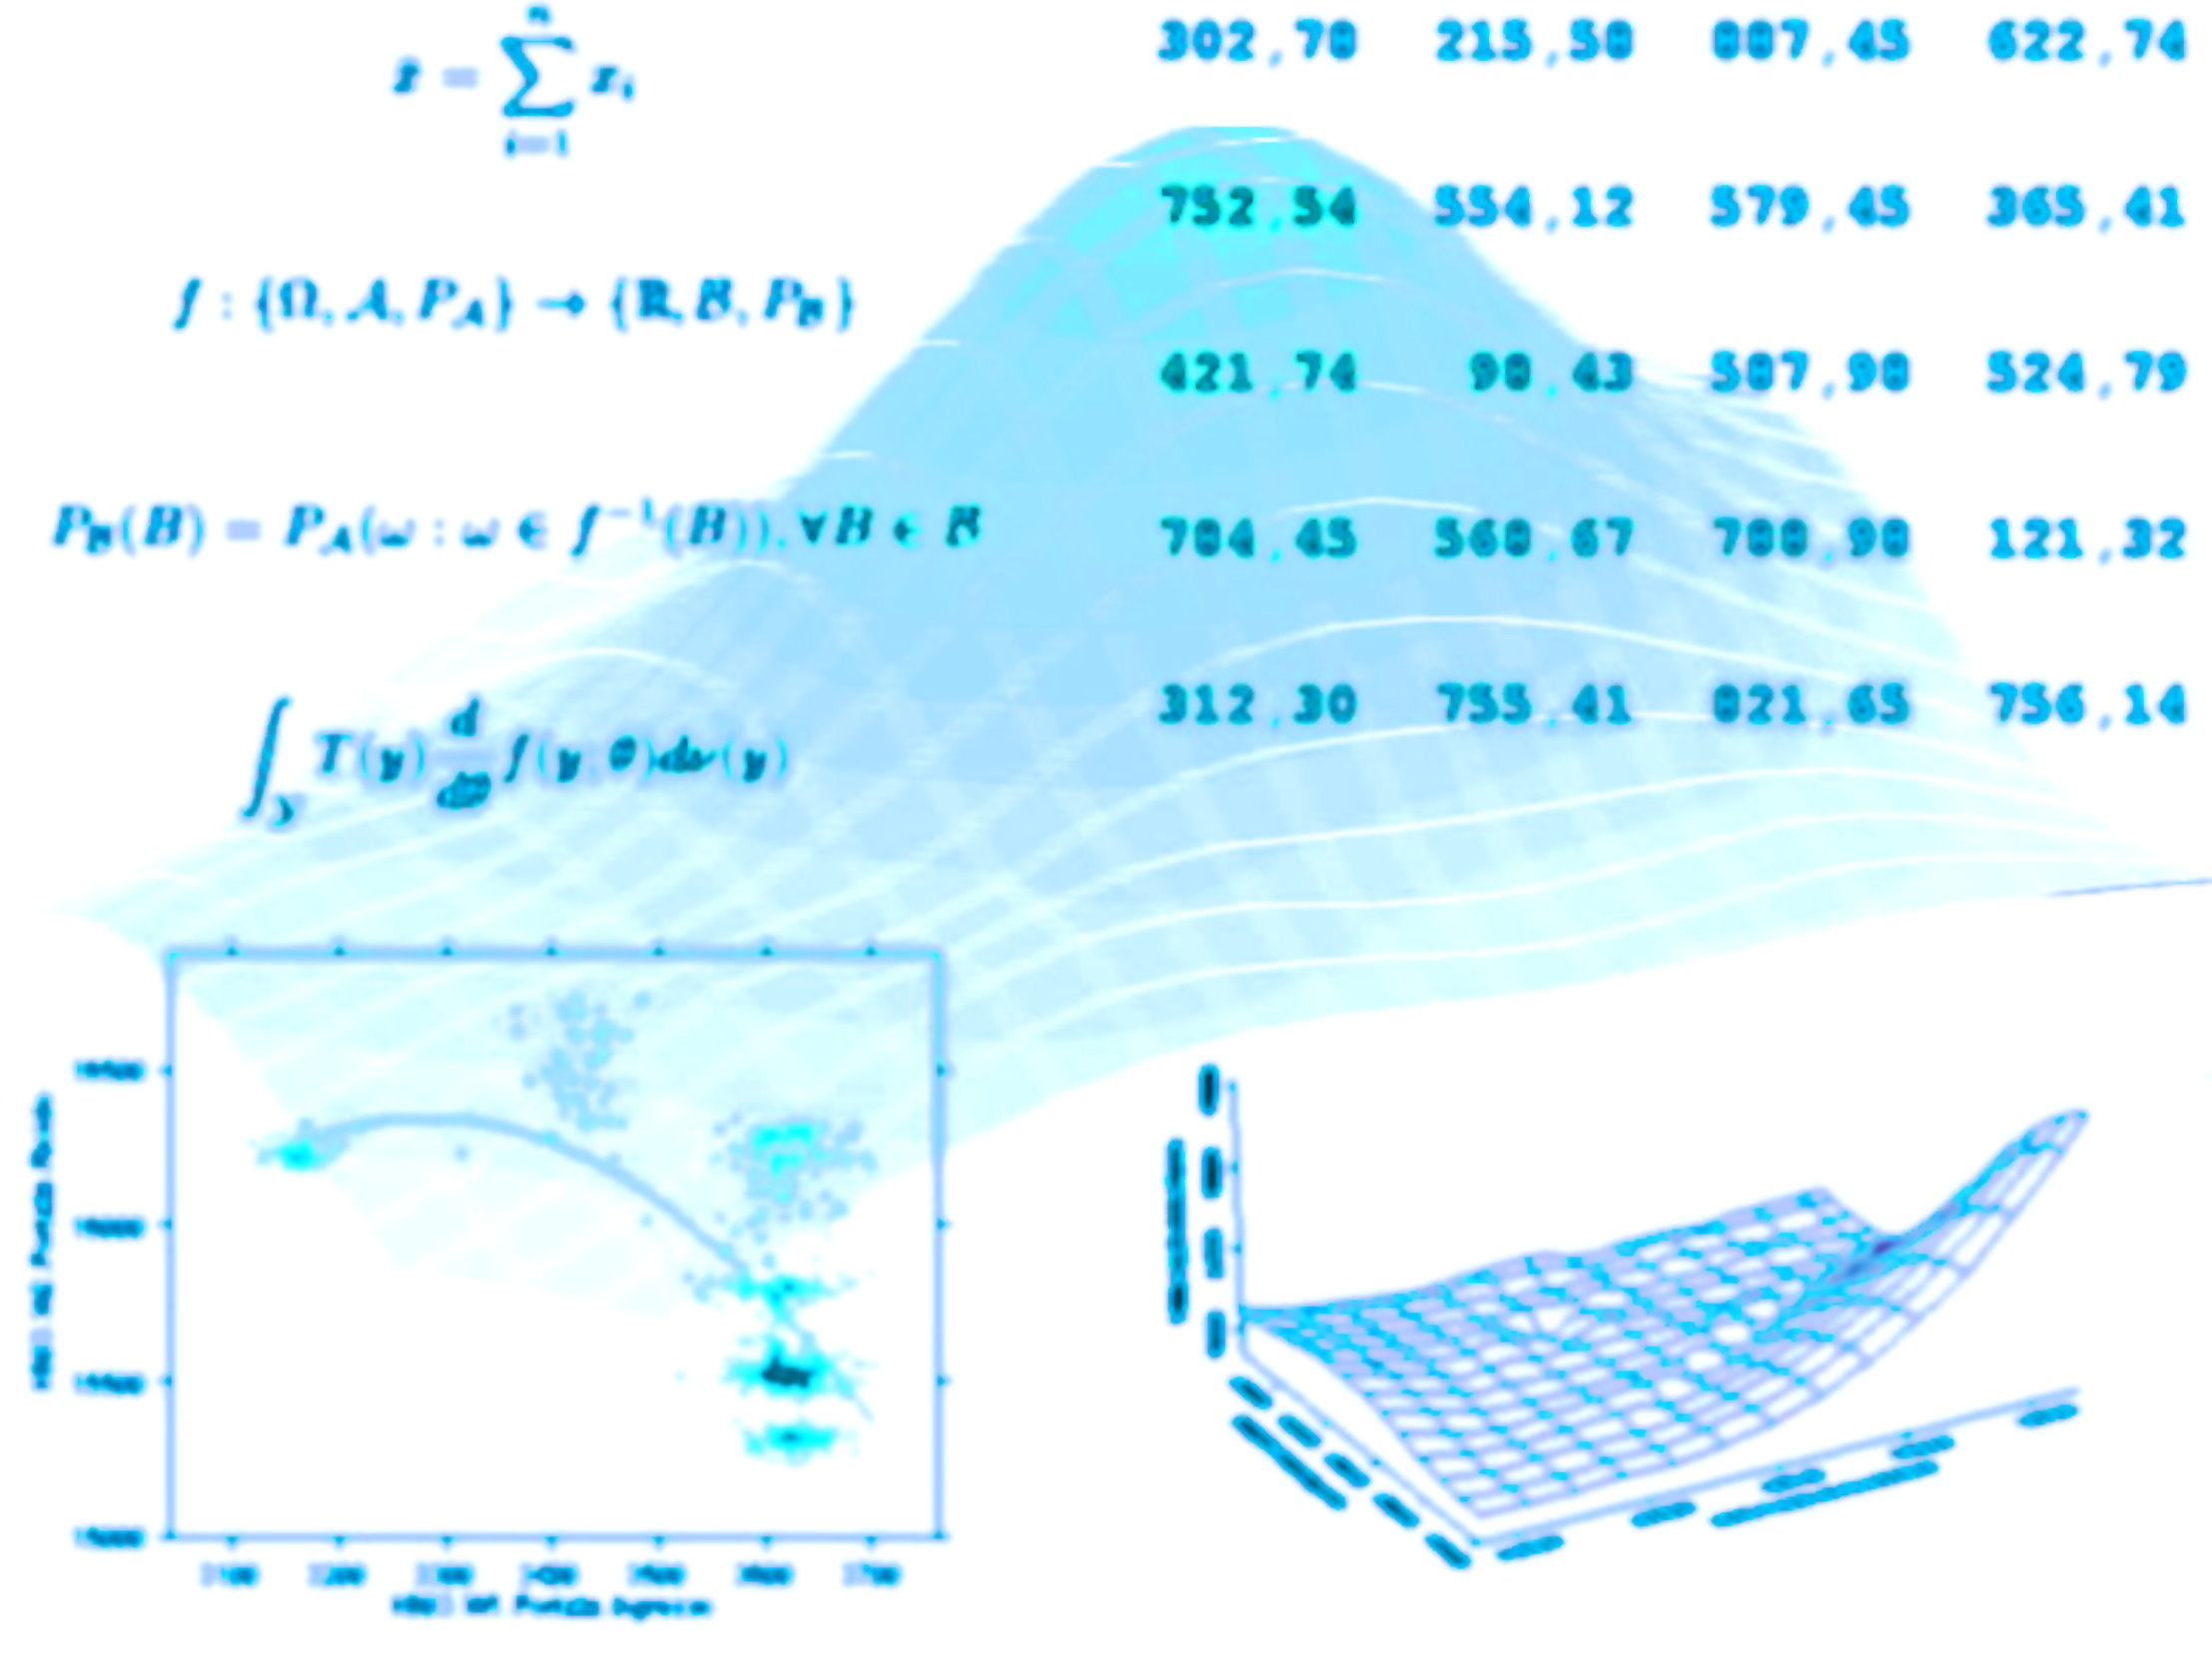
\includegraphics[width=.70\textwidth, height=11cm, keepaspectratio=false]{img/titolo2.png}
    \centering
  \end{figure}
\end{figtitolo}}



\definecolor{ablue}{rgb}{0.729, .824, .878}  % azzurro
\definecolor{iblue}{rgb}{0.0235294117647059,0.282352941176471,0.47843137254902}  % azzurro
\definecolor{ared}{rgb}{0.671,0.161,0.18}
% info box principale per prop e teoremi

\newtcolorbox{info}{
%beamer,
enhanced,
breakable,
colupper=iblue,
%frame style={upper left=blue,upper right=red,lower left=yellow,lower right=green},
colback=white!50!ablue,
%colframe=ablue,
%colframe=ablue!90!black,
width=\linewidth,
arc=0.1mm,
 boxsep=0mm,
 left=15mm,
left*=2mm,
%interior style={top color=iblue!10!white,middle color=iblue!20!white,bottom color=iblue!30!white},
interior style={top color=iblue!8!white,middle color=iblue!10!white,bottom color=iblue!12!white},
boxrule=0pt,
drop fuzzy shadow
}


\newtcolorbox{info2}{
enhanced,
colupper=iblue,
colback=white!50!ablue,
width=\linewidth,
arc=0.1mm,
 boxsep=0mm,
 left=15mm,
left*=2mm,
interior style={top color=iblue!8!white,middle color=iblue!10!white,bottom color=iblue!12!white},
boxrule=0pt,
drop fuzzy shadow
}

% info box con attenzione
\newenvironment{att}
  {
\begin{tcolorbox}[enhanced,arc=0.1mm,boxrule=1pt,colback=white,colframe=ared,title=\bf\small \fontfamily{lmss}\selectfont \faExclamationTriangle \hspace{.5 cm} Attenzione,drop fuzzy shadow]
}{
\end{tcolorbox}
  }
% info box con nota
\newenvironment{nota}
  {
\begin{tcolorbox}[enhanced,breakable,arc=0.1mm,boxrule=1pt,colback=white,colframe=iblue,title=\bf \fontfamily{lmss}\selectfont \faInfoCircle \hspace{.5 cm} Nota,drop fuzzy shadow]
}{
\end{tcolorbox}
  }

% per escludere le soluzioni togliere il commento a \excludecomment{sol} 
%
% \excludecomment{sol} 
% 
% e commentare da qui ↓

% info box con Soluzione

\newenvironment{sol}
  {
  \begin{tcolorbox}[enhanced,breakable,arc=0.1mm,boxrule=1pt,colback=white,colframe=iblue,
  title=\bf \fontfamily{lmss}\selectfont \hspace{.5 cm} Soluzione,drop fuzzy shadow]

}{
\end{tcolorbox}
  }

% a qui ↑ 

\newtcolorbox{titolo}{
enhanced,
beforeafter skip=0pt,
colupper=white,
colback=iblue,
width=\paperwidth,
arc=0.0mm,
boxsep=1mm,
%left=-2cm,
left*=-5cm,
boxrule=0pt,
grow to left by=3cm,
%grow to right by=3cm,
%enlarge right by=2cm
%drop fuzzy shadow
}

\newtcolorbox{figtitolo}{
enhanced,
beforeafter skip=0pt,
colupper=white,
colback=white,
width=\paperwidth,
arc=0.0mm,
boxsep=1mm,
%left=-2cm,
left*=-5cm,
boxrule=0pt,
%grow to left by=3cm,
%grow to right by=3cm,
%enlarge right by=2cm
%drop fuzzy shadow
}

\newenvironment{minip}
  {
\begin{tcolorbox}[enhanced, breakable,
left skip=1cm,
right skip=1cm,
%width=0.5\linewidth,
 % boxsep=5mm,
 % left=-15mm,
 % left*=20mm,
 arc=0mm,
boxrule=1pt,
colback=white,
drop fuzzy shadow]
}{
\end{tcolorbox}
  }

  
% definisco il comando mc che crea un cerchio intorno ad un carattere: di prossima soppresisone
\makeatletter
\newcommand\mc[1]{%
  \mathpalette\@mc{#1}%
}
\newcommand\@mc[2]{%
  \tikz[baseline=(math.base)] \node[draw,circle,inner sep=1pt] (math) {$\m@th#1#2$};%
}
\makeatother




% Roba vecchia


% qui di definisce quanti oggetti flottanti devono andare
% nella parte alta della pagine, nella bassa, ecc.
% meglio non toccare niente perché si fa un casino micidiale
% \renewcommand{\topfraction}{.35}
% \renewcommand{\bottomfraction}{.35}
% \renewcommand{\textfraction}{.50}
% \renewcommand{\floatpagefraction}{.99}
% \setcounter{topnumber}{1}
% \setcounter{bottomnumber}{2}
%\setcounter{totalnumber}{2}


% \newtheorem{thm}{Theorem}[section]
% \renewcommand{\thethm}{\arabic{section}.\textbf{\sffamily\arabic{thm}}}

% \newtcolorbox{info2}{
%   colback=black,
%   colframe=orange,
%   coltext=white,
%   boxsep=5pt,
%   arc=4pt}

%\definecolor{ablue}{rgb}{0.36, 0.54, 0.66} blue air

%\usepackage{tocloft}
%\usepackage{thmtools}

%\setlength{\fboxsep}{.4em}

% \newenvironment{info}{
%   \definecolor{shadecolor}{rgb}{0.729, .824, .878}  % azzurro
%   
% %  \definecolor{shadecolor}{rgb}{.9, .9, .9}  % grigio  
%   %\color{white}
%   \begin{shaded}}
%  {\end{shaded}}
 
% \newtcolorbox{nota}{
% colupper=black!75!blue,
% %frame style={upper left=blue,upper right=red,lower left=yellow,lower right=green},
% colback=white,
% colframe=red!75!black,
% %colframe=ablue!90!black,
% width=\linewidth,
% arc=0.5mm,
%  boxsep=0mm,
%  left=15mm,
% left*=2mm
% }

%\tcbuselibrary{all}
% \newtcolorbox{info2}{
% beamer,
% colback=yellow,
% colframe=orange,
% colupper=red,
% %colframe=ablue!90!black,
% width=\linewidth,
% arc=10mm,
%  boxsep=0mm,
%  left=15mm,
% left*=5.5mm
% }


